\subsection*{Problema 46}
\textbf{Enunciado:} Calcular la integral:
\begin{align*}
\int (4x^2 + 4x - 3)^{-1/2} \, dx
\end{align*}

\textbf{Solución:}
Primero, expresamos la integral con el radical en el denominador:
\begin{align*}
\int \dfrac{1}{\sqrt{4x^2 + 4x - 3}} \, dx
\end{align*}

Completamos el cuadrado en el trinomio dentro de la raíz. Factorizamos el coeficiente principal del término cuadrático:
\begin{align*}
4x^2 + 4x - 3 &= 4\left(x^2 + x - \dfrac{3}{4}\right)
\end{align*}

Completamos el trinomio cuadrado perfecto sumando y restando $(1/2)^2 = 1/4$:
\begin{align*}
4\left[\left(x^2 + x + \dfrac{1}{4}\right) - \dfrac{1}{4} - \dfrac{3}{4}\right] &= 4\left[\left(x + \dfrac{1}{2}\right)^2 - 1\right]
\end{align*}

Distribuimos el factor $4$:
\begin{align*}
4\left(x + \dfrac{1}{2}\right)^2 - 4 &= (2x + 1)^2 - 4
\end{align*}

Sustituimos la expresión completada en la integral original:
\begin{align*}
\int \dfrac{1}{\sqrt{(2x + 1)^2 - 4}} \, dx
\end{align*}

Realizamos la sustitución: sea $u = 2x + 1$, de donde $du = 2 \, dx$, lo que implica que $dx = \frac{1}{2} \, du$. La integral se transforma en:
\begin{align*}
\dfrac{1}{2} \int \dfrac{1}{\sqrt{u^2 - 4}} \, du
\end{align*}

Utilizamos la fórmula estándar de integración para funciones con radicales de la forma $\sqrt{u^2 - a^2}$:
\begin{align*}
\int \dfrac{1}{\sqrt{u^2 - a^2}} \, du = \ln\left|u + \sqrt{u^2 - a^2}\right| + C
\end{align*}

Aplicando la fórmula con $a = 2$:
\begin{align*}
\dfrac{1}{2} \ln\left|u + \sqrt{u^2 - 4}\right| + C_1
\end{align*}

Regresamos a la variable original $x$ sustituyendo $u = 2x + 1$:
\begin{align*}
\dfrac{1}{2} \ln\Big|2x + 1 &+ \sqrt{(2x + 1)^2 - 4}\Big| + C_1
\end{align*}

Simplificamos el argumento dentro del radical para obtener la forma final:
\begin{align*}
\dfrac{1}{2} \ln\Big|2x + 1 &+ \sqrt{4x^2 + 4x - 3}\Big| + C
\end{align*}

\begin{figure}[H]
	\centering
	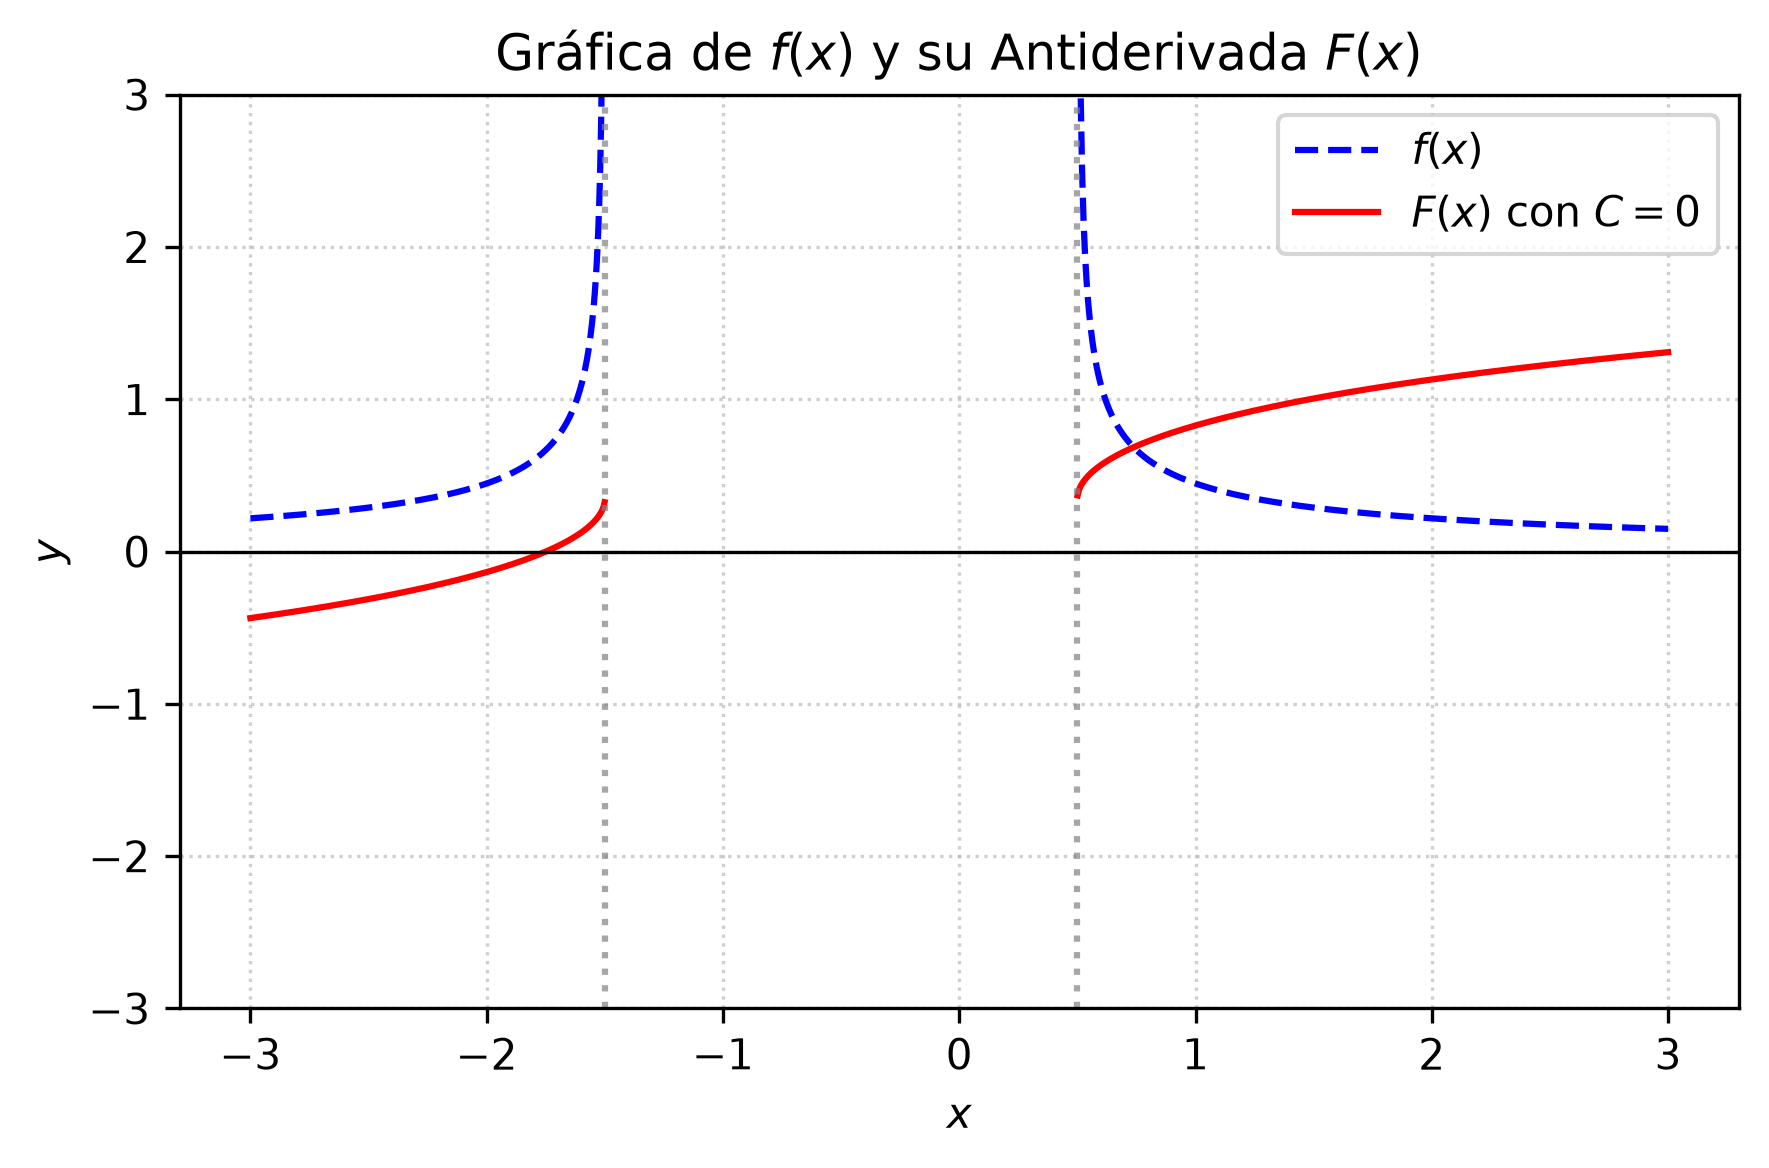
\includegraphics[width=\columnwidth]{semana_05/graficas/SEM05_P46_grafica.png}
	\caption{Representación gráfica de $f(x)$ y su antiderivada $F(x)$ evaluada para la constante de integración $C = 0$ (Problema 46).}
	\label{fig:problema46}
\end{figure}
